%----------------------------------------------------------------------------------------
%	PACKAGES AND THEMES
%----------------------------------------------------------------------------------------
\documentclass[aspectratio=169,xcolor=dvipsnames]{beamer}
\usetheme{Simple}
\usepackage[fixed]{fontawesome5}
\usepackage{hyperref}
\usepackage{graphicx} % Allows including images
\usepackage{booktabs} % Allows the use of \toprule, \midrule and \bottomrule in tables

%----------------------------------------------------------------------------------------
%	TITLE PAGE
%----------------------------------------------------------------------------------------

% The title
\title[short title]{Use and Misuse of Continuous Integration Features}
\subtitle{An Empirical Study of Projects that (mis)use Travis CI}

\author[Pin-Yen] {Authors: Keheliya Gallab and Shane McIntosh }

\institute[NTU] % Your institution may be shorthand to save space
{   Philip Mottershead
    % Your institution for the title page
    % Department of Computer Science and Information Engineering \\
    % National Taiwan University 
    \vskip 3pt
}
\date{February 15 2021} % Date, can be changed to a custom date


%----------------------------------------------------------------------------------------
%	PRESENTATION SLIDES
%----------------------------------------------------------------------------------------

\begin{document}
\begin{frame}
    % Print the title page as the first slide
    \titlepage
\end{frame}
\begin{frame}{Authors}
    \begin{columns}[c] % The "c" option specifies centered vertical alignment while the "t" option is used for top vertical alignment
        \column{.5\textwidth} % Left column and width
        \begin{figure}
            \centering
            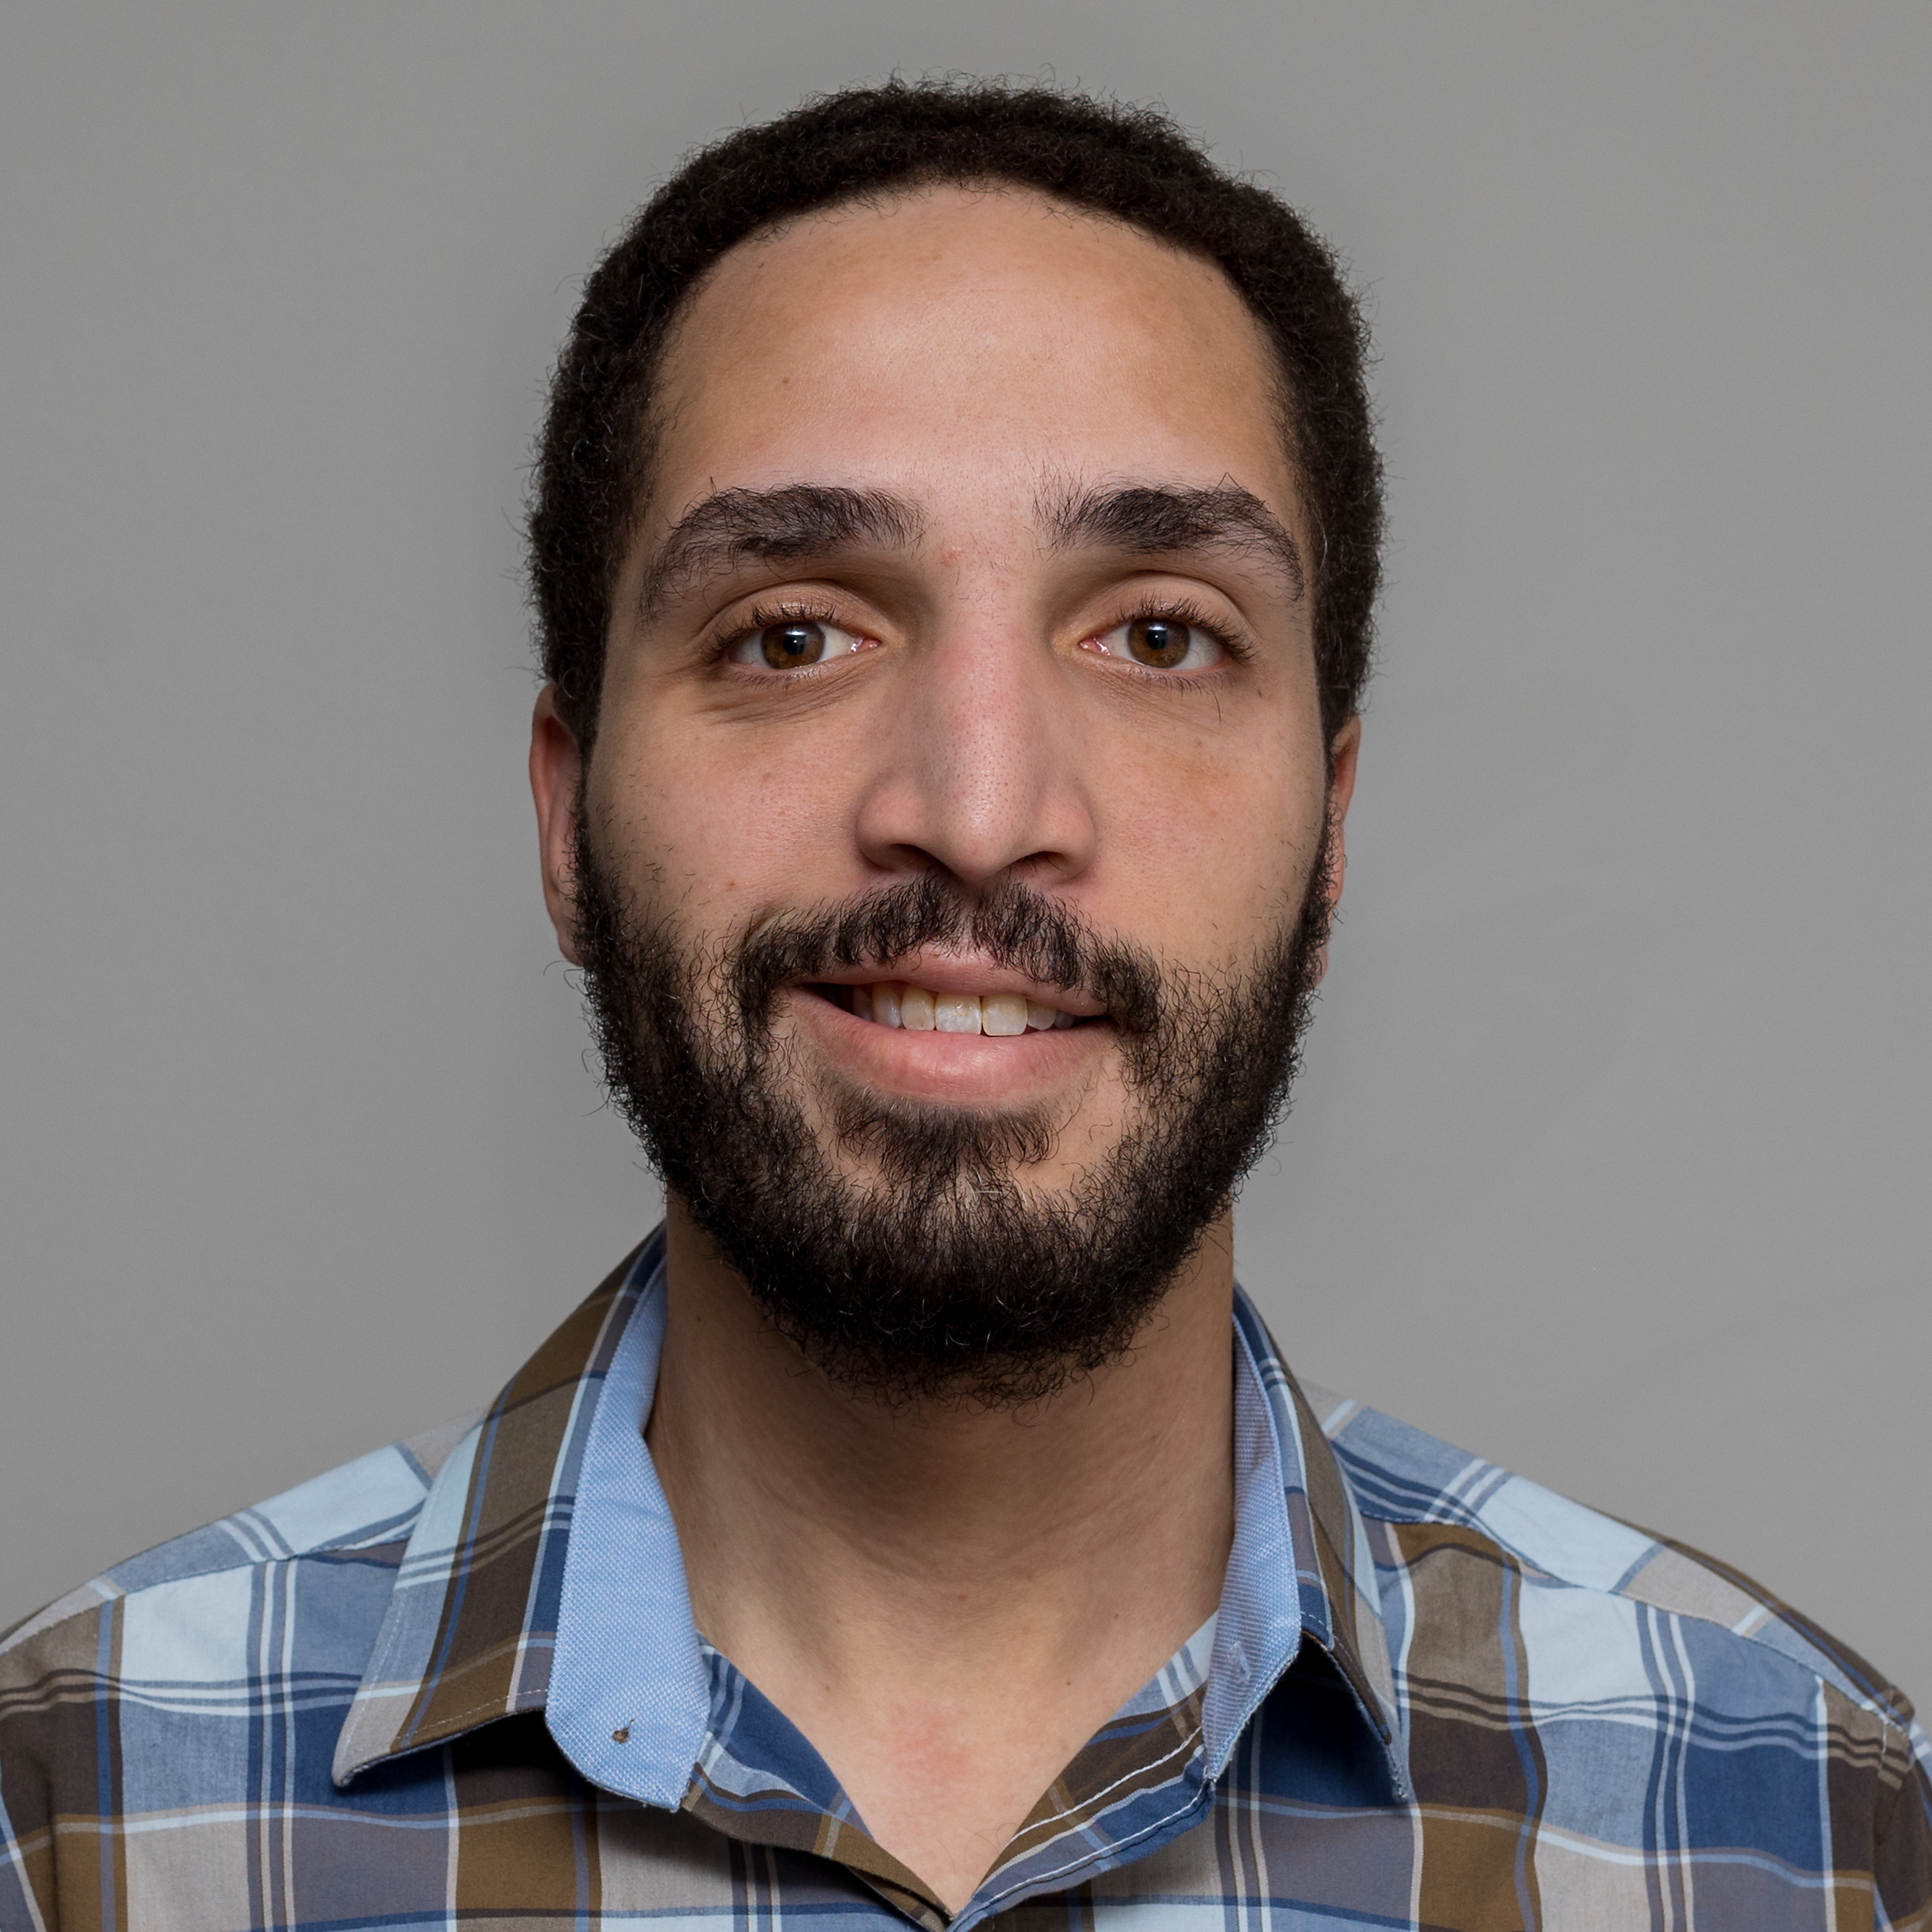
\includegraphics[width=0.5\textwidth]{images/shane.jpg}
            \label{fig:my_label}
        \end{figure}
        \centering{Shane McIntosh}\linebreak
        \centering Assistant Professor \linebreak    
        \centering{McGill University, Canada}
        \centering\url{http://rebels.ece.mcgill.ca/}

        \column{.5\textwidth} % Right column and width
       \begin{figure}
           \centering
           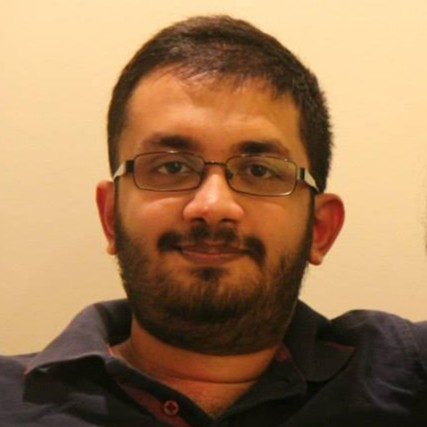
\includegraphics[width=0.5\textwidth]{images/keheliya.jpg}
           \label{fig:my_label}
       \end{figure}
       \centering{Keheliya Gallab}\linebreak
       \centering PhD student \linebreak
       \centering{McGill University, Canada}
       \centering \url{https://keheliya.github.io/}

    \end{columns}
\end{frame}
\begin{frame}{Presenter}
    \begin{figure}
        \centering
        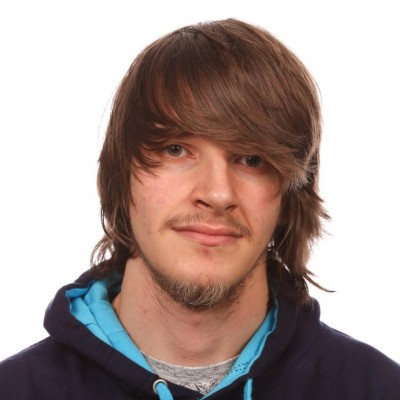
\includegraphics[width=0.25\textwidth]{images/index.jpg}
        \label{fig:my_label}
    \end{figure}
    \centering Philip Mottershead\linebreak
    \centering MEng Software Engineering\linebreak
    \centering Aberystwyth University \linebreak
    \centering phm14@aber.ac.uk\linebreak
\end{frame}


\begin{frame}{Overview}
    % Throughout your presentation, if you choose to use \section{} and \subsection{} commands, these will automatically be printed on this slide as an overview of your presentation
    \tableofcontents
\end{frame}

%------------------------------------------------
\section{Modern-CI-Process}
%------------------------------------------------

\begin{frame}{Continuous Integration}
    \begin{itemize}
        \item Continuous integration (CI) is the process of merging small changes often and automating the build and test process.
        \item Continuous deployment (CD) is the process of automating the deployment process
        \item Several tools create what is known as the CI/CD pipeline
    \end{itemize}

     \begin{itemize}
            \item Self Hosted
            \begin{itemize}
                \item \href{https://docs.gitlab.com/ee/ci/}{Jenkins \faExternalLink*}
                \end{itemize}
            \item VCS based
            \begin{itemize}
                \item \href{https://docs.gitlab.com/ee/ci/}{Gitlab CI \faExternalLink*}
                \item \href{https://github.com/features/actions}{GitHub Actions \faExternalLink*}
            \end{itemize}
            \item Cloud hosted
            \begin{itemize}
                \item \href{https://travis-ci.com/} {Travis CI \faExternalLink*} 
                \item \href{https://circleci.com/} {Circle CI \faExternalLink*}
            \end{itemize}
        \end{itemize}
\end{frame}

\begin{frame}{Overall Infrastructure}
    \begin{figure}
        \centering
        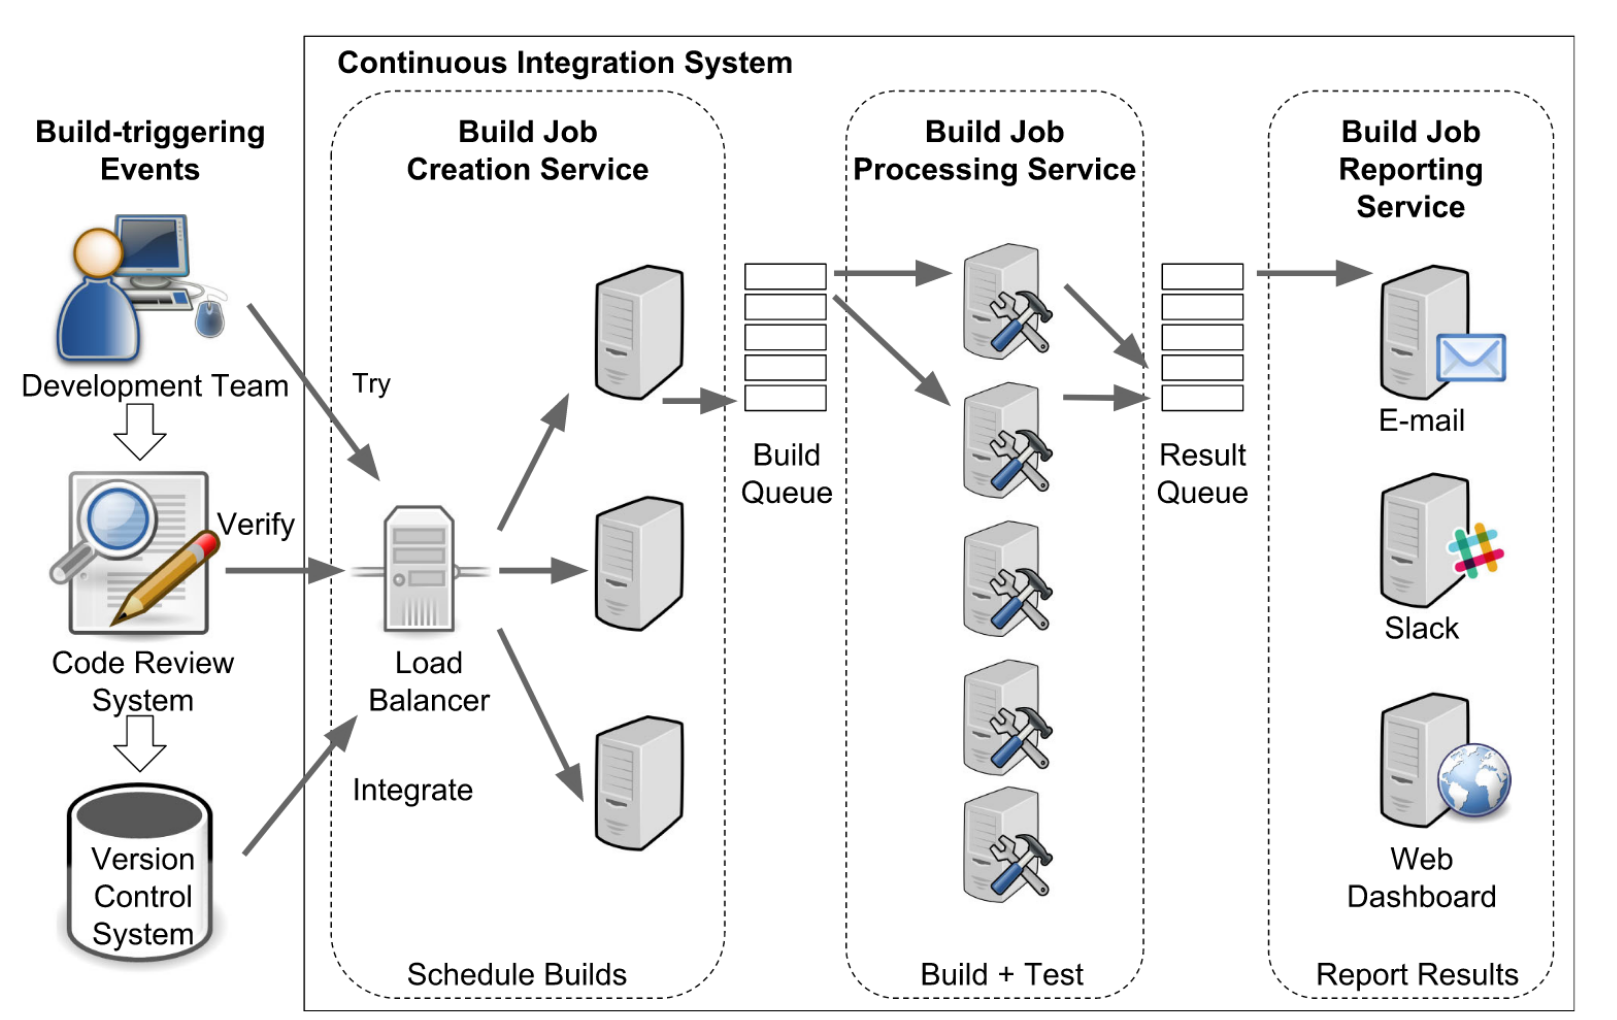
\includegraphics[width=0.7\textwidth]{images/infrastucture.png}
        \label{fig:my_label}
    \end{figure}
\end{frame}

\begin{frame}{Travis CI}

\begin{itemize}
    \item \url{https://travis-ci.org/}
    \item Cloud hosted continuous integration service
    \item Founded in 2011 in Berlin, Germany
    \item 50\% of third party CI tool usage on Github is Travis CI  \cite{noauthor_github_2017}
    
\end{itemize}
         \begin{figure}
            \centering
            
\includegraphics[width=0.25\textwidth]{images/TravisCI-Mascot-1.png}
            \label{fig:my_label}
        \end{figure}
\end{frame}

%------------------------------------------------
\section{Configuring-Travis-CI}
%------------------------------------------------


\begin{frame}{Travis CI Configuration}
    \begin{itemize}
        \item Configuration files are in YAML
        \item Stored in .travis.yml in your repository
        \item Split into two main sections
        \begin{itemize}
            \item Node Configuration
            \item Build Process Configuration 
            \begin{itemize}
                \item Install Phase
                \item Script Phase
            \end{itemize}
        \end{itemize}
    \end{itemize}
    \begin{figure}
        \centering
        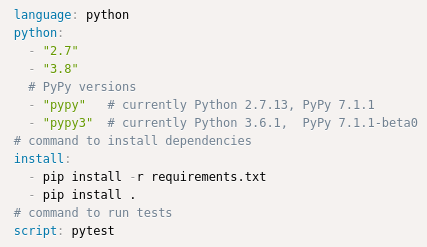
\includegraphics[width=0.45\textwidth]{images/Screenshot_20210212_211355.png}
        \label{fig:my_label}
    \end{figure}
\end{frame}

\begin{frame}{Node configuration}
    \begin{figure}
        \centering
        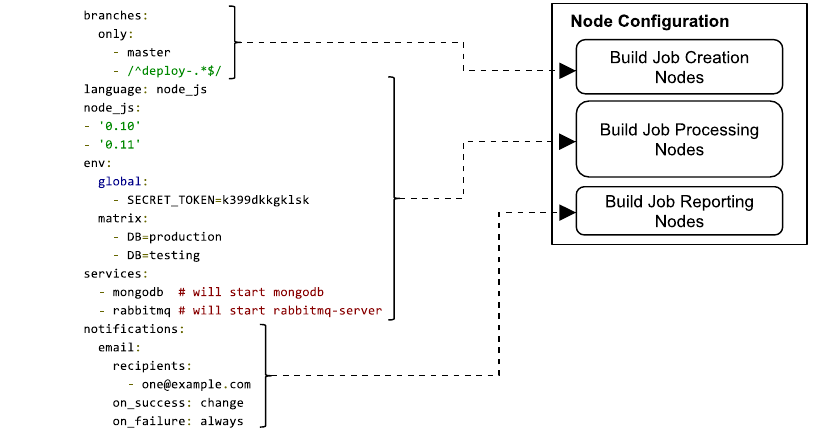
\includegraphics[width=0.8\textwidth]{images/Node Configuration.png}
        \label{fig:my_label}
    \end{figure}
\end{frame}

\begin{frame}{Install Phase}
    \begin{figure}
        \centering
        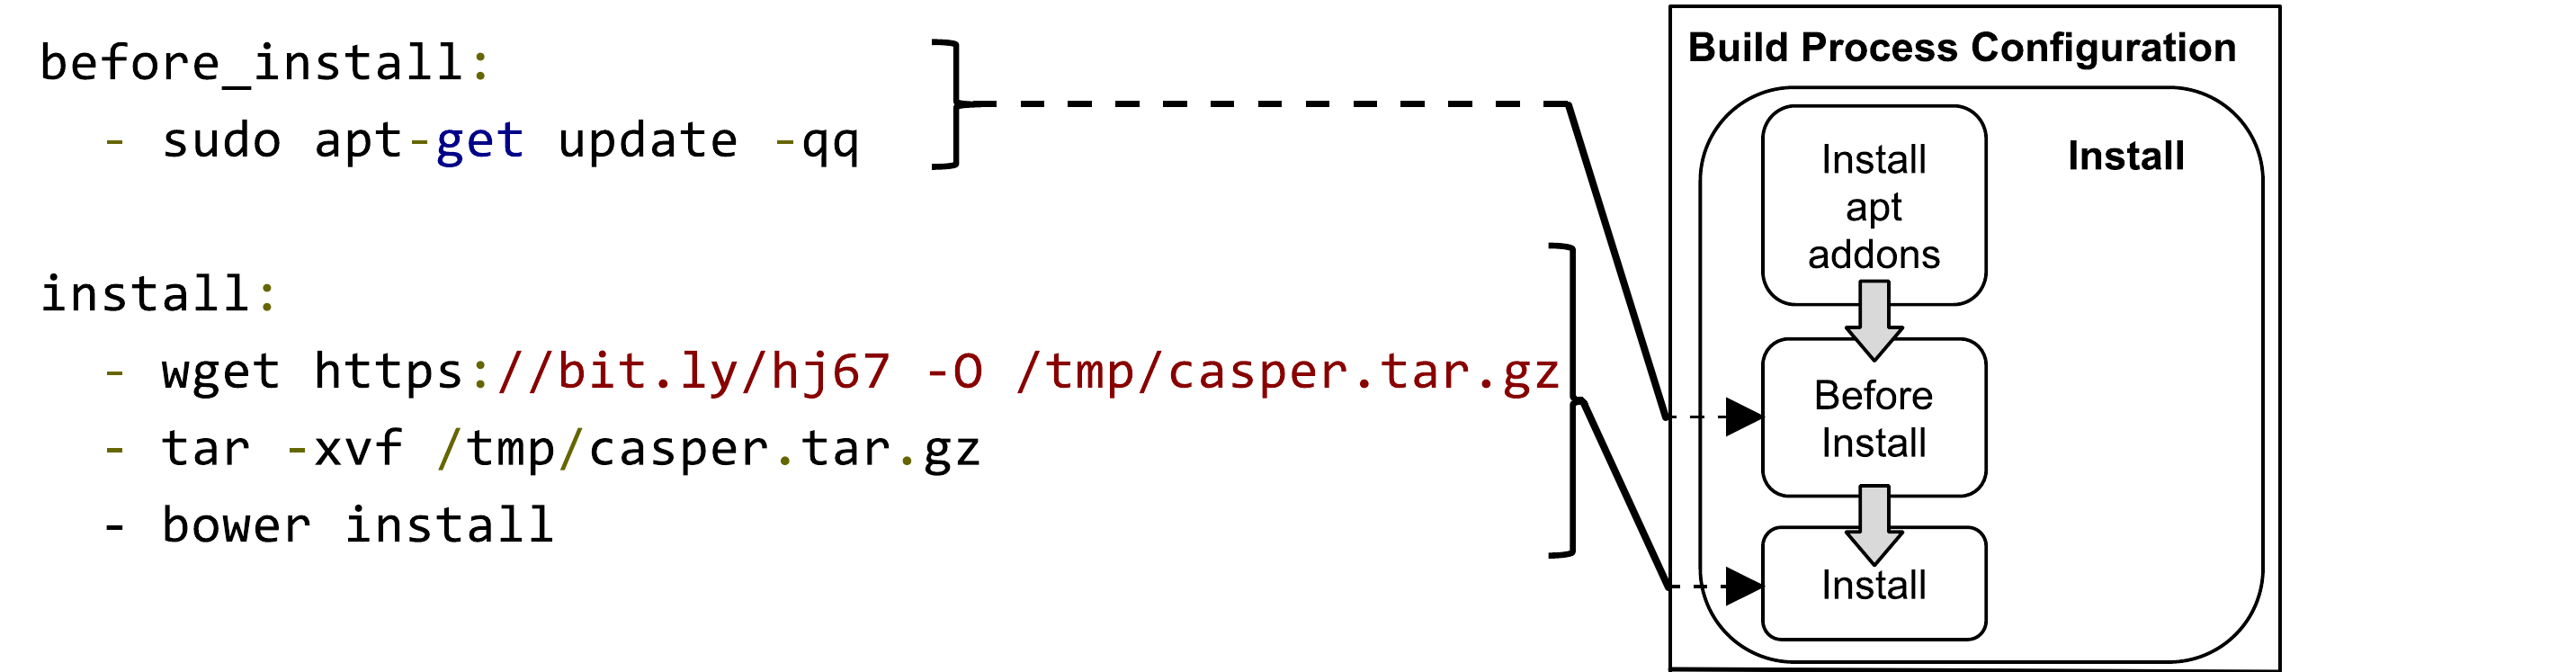
\includegraphics[width=0.9\textwidth]{images/install.png}
        \label{fig:my_label}
    \end{figure}
\end{frame}

\begin{frame}{Script Phase}
    \begin{figure}
        \centering
        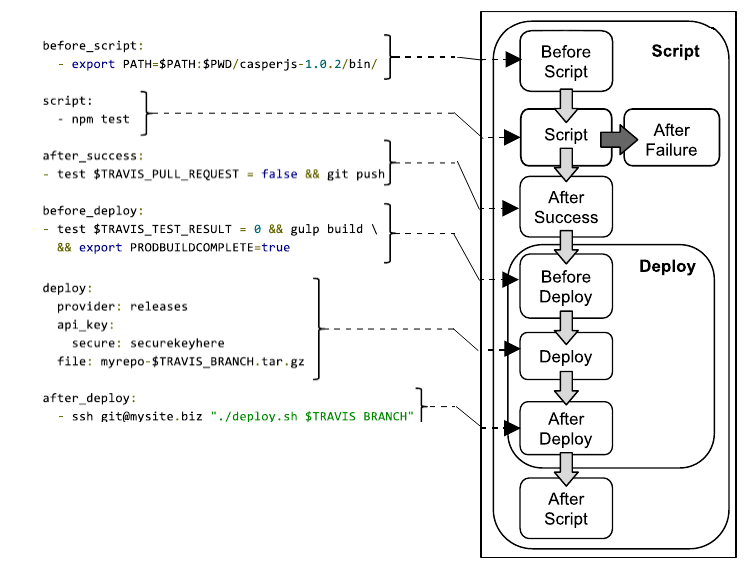
\includegraphics[width=0.6\textwidth]{images/Script_phase.png}
        \label{fig:my_label}
    \end{figure}
\end{frame}


%------------------------------------------------
\section{Travis-CI-Usage-Study}
%------------------------------------------------
\begin{frame}{Travis CI Usage Study}
    \begin{enumerate}
        \item Rational for Github
        \item Data Filtering
        \item Commonly used languages
        \item Configuration Statement distribution
        \item Change in Configuration files
    \end{enumerate}
\end{frame}
\begin{frame}{Rational for Github}
    \begin{itemize}
        \item Need large and diverse set of projects
        \item Query data on GitHub dataset on Google BigQuery
        \begin{itemize}
            \item Number of commits
            \item Number of files
        \end{itemize}
        \item Query returned 
        \begin{itemize}
            \item 2,911,522 repositories
    %         \item 4,022,651,601 commits 
		  %  \item 2,133,880,097 files
        \end{itemize}
    \end{itemize}
\end{frame}

\begin{frame}{Data Filtering}
    \begin{enumerate}
        \item Filter based on commit(100) and file(500) thresholds
        \item Filter for projects with a .travis.yml file
        \item Filter for projects not flagged as forks by Github API
        \item Filter for projects with similarity less that 70\% based on commit hashes
    \end{enumerate}

    \begin{figure}
        \centering
        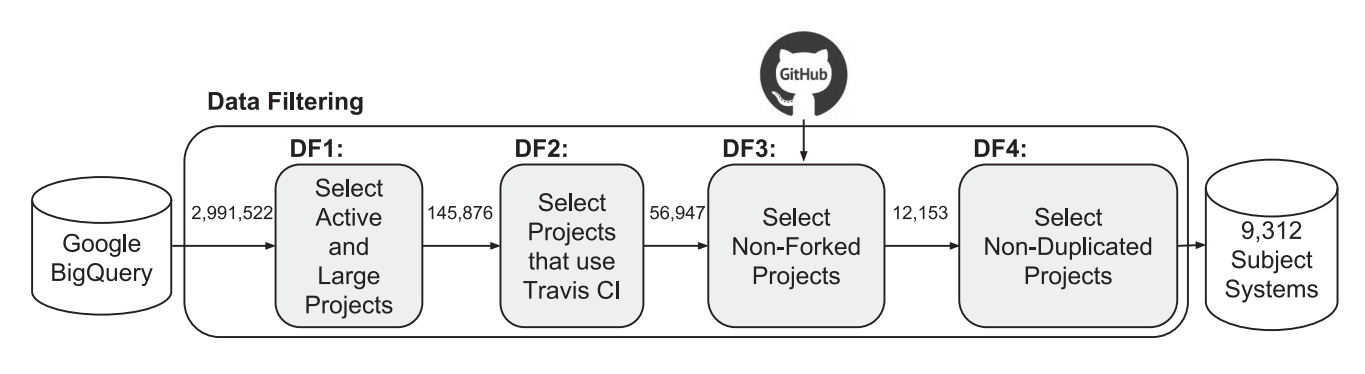
\includegraphics[width=0.8\textwidth]{images/data-filtering.png}
        \label{fig:my_label}
    \end{figure}
\end{frame}

\begin{frame}{Commonly used languages}
\begin{itemize}
    \item Checks the language property in .travis.yml
    \item Most common is language is Node.js
    \item Similar to results language usage surveys \\
    
    % \begin{itemize}
    %     \item Stack overflow\cite{noauthor_stack_nodate}
    %     \item Github \cite{noauthor_state_nodate}
    % \end{itemize}
            \centering
            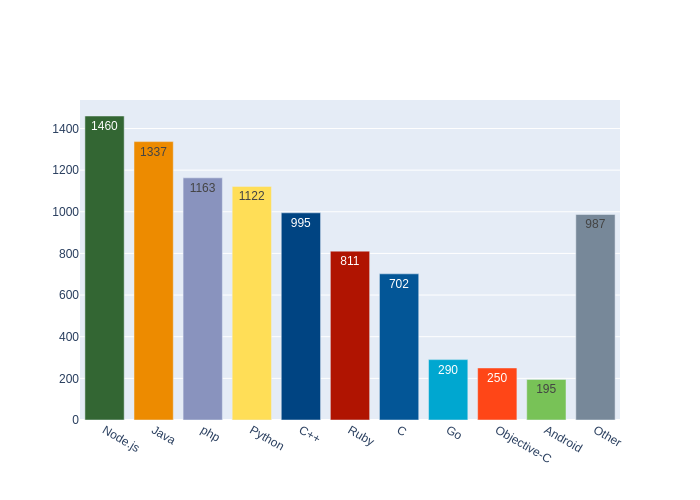
\includegraphics[width=0.535\textwidth]{images/fig21.png}
\end{itemize}

\end{frame}

\begin{frame}{Configuration Statement distribution}
    \begin{itemize}
        \item Spread of configuration code
        \item Quantity of code in each section
        \item Label each property in .travis.yml related to build process
        \item Divided into 4 sub categories
        \begin{itemize}
            \item Build job creation
            \item Build job processing
            \item Build status notification
            \item Other 
        \end{itemize}
        \item Count the lines in each section of each file
    \end{itemize}
\end{frame}
\begin{frame}{Configration statements}
    \begin{figure}
        \centering
        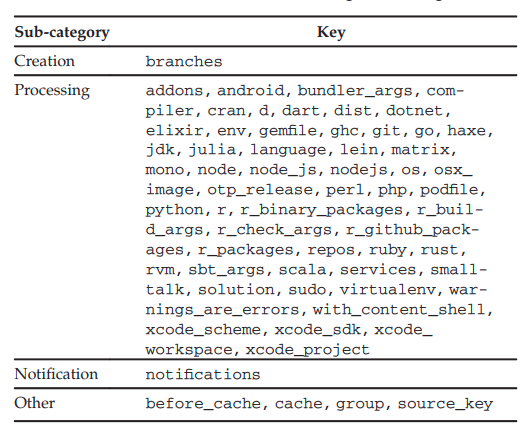
\includegraphics[width=0.5\textwidth]{images/Section-Labels.png}
        \label{fig:my_label}
    \end{figure}
\end{frame}
\begin{frame}{Statement statistics}
    \begin{itemize}
        \item CI Job Processing jobs in 95\% of projects
        \begin{itemize}
            \item 48\% of all config code
        \end{itemize}
        \item script phase in 76\% of projects 
        \begin{itemize}
            \item 12\% of all config code
        \end{itemize}
    \end{itemize}
      \begin{figure}
        \centering
        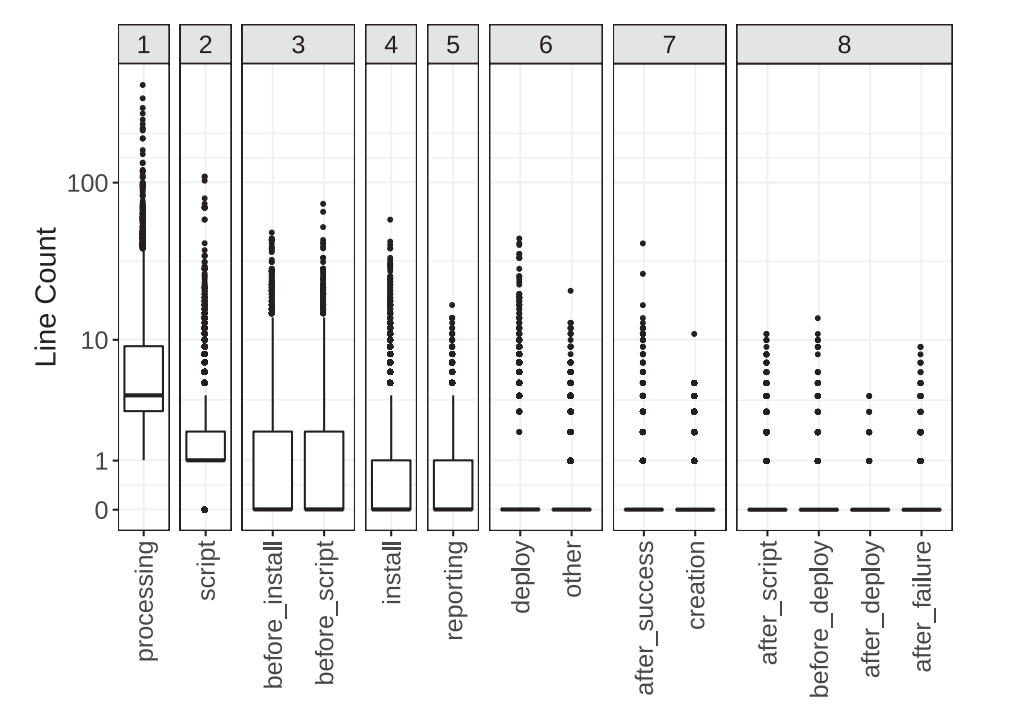
\includegraphics[width=0.49\textwidth]{images/Line-count-distribution.png}
        \label{fig:my_label}
    \end{figure}
\end{frame}
\begin{frame}{Change in Configuration files}
    \begin{itemize}
        \item Count number of commits that modify the the .travis.yml file
        \item Using Line to section mapping we match line changes to the section of the file
    \end{itemize}
    \end{frame}
\begin{frame}{Change in Configuration files}
    \begin{itemize}
        \item 18 times on average
        \item max of 366
        \item More that 75\% modified fewer than 10 times
        \item Most common is Processing section
    \end{itemize}
    \begin{figure}
        \centering
        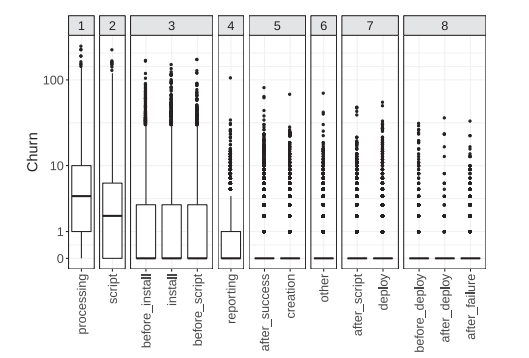
\includegraphics[width=0.5\textwidth]{images/Churn.png}
        \label{fig:my_label}
    \end{figure}
\end{frame}


%------------------------------------------------
\section{Travis-CI-Anti-Patterns}
%------------------------------------------------
\begin{frame}{Anti-Pattern Study}

    \begin{itemize}
        \item Anti-Patterns
        \item Hansel and Gretel 
        \item Anti-Patterns Selected
        \begin{itemize}
            \item Bypassing Security Checks Motivation
            \item Using Irrelevant Properties
            \item Commands Unrelated to the Phase
        \end{itemize}
        \item Results of study
        \begin{itemize}
            \item Prevalence of anti-patterns
            \item Automatic removal of anti-patterns
            \item Acceptance of Automatic removals
        \end{itemize}
    \end{itemize}
\end{frame}
\begin{frame}{Anti-Patterns}
    \begin{itemize}
        \item We Define CI spec for anti-patterns as violations of best practices
        \begin{itemize}
            \item 
        \end{itemize}
    \end{itemize}
    - Could have unintended consequences
	-  broken or incorrect builds
	- Maintenance issues
	- Comprehensibility issues
- TRAVIS LINT
	- scans .travis.yml files for mistakes
	- common pitfalls
	- formatting issues, missing mandatory fields
	-  can prevent configuration errors from breaking project builds.
\end{frame}

\begin{frame}{Hansel and Gretel}
    
\end{frame}
\begin{frame}{Anti-Patterns Selected}
    
\end{frame}

\begin{frame}{Redirecting Scripts into Interpreters}
    
\end{frame}

\begin{frame}{Redirecting Scripts into Interpreters}
    
\end{frame}

\begin{frame}{Bypassing Security Checks Motivation}
    
\end{frame}

\begin{frame}{Using Irrelevant Properties}
    
\end{frame}

\begin{frame}{Commands Unrelated to the Phase}
    
\end{frame}

\begin{frame}{Prevalence of anti-patterns}
    
\end{frame}

\begin{frame}{Automatic removal of anti-pattern}
    
\end{frame}

\begin{frame}{Acceptance of Automatic removals}
    
\end{frame}

%------------------------------------------------
\begin{frame}[allowframebreaks]{References}
\def\newblock{}

\bibliographystyle{ieeetr}
\bibliography{references}
\end{frame}

\begin{frame}
    \Huge{\centerline{The End}}
\end{frame}

%----------------------------------------------------------------------------------------

\end{document}